\section{ACL en use}

Dans cette session on verrais les uses des ACL dans les système d'aujourd'hui. 

\subsection{ACL Kernel Patches}
Les ACL \emph{patches} ont été ajouter dans le noyaux Linux depuis November 2002. Cette \emph{patches} implémentent le POSIX 1003.1e brouillon 17 et elle ont été ajoute dans le version 2.5.46. Donc le support ACL et aussi présent dans le dernière version du noyaux aujourd'hui. Depuis 2004 le support aux ACL étions disponible pour les système de fichier Ext2, Ext3, IBM JFS, ReiserFS et SGI XFS. Les ACL sont supporte aussi pour le système NFS, par contre, il y a quelques problèmes de sécurité connu\cite{nfs_problem}. 

Aujourd'hui c'est assez simple pour ajouter le supporte aux ACL dans les distribution Linux comme Ubuntu ou Debian. On verrais les pas pour ajouter ce supporte après.

\subsection{Mac OSX}
Le système de exploitation Mac OSX (10.6.2 Snow Leopard dans le moment de écriture de ce article) a aussi les supporte aux ACL complètement intégrée dans l'interface de utilisateur (\ref{fig:img_mac-acl}). 

\begin{figure}[htbp]
	\centering
		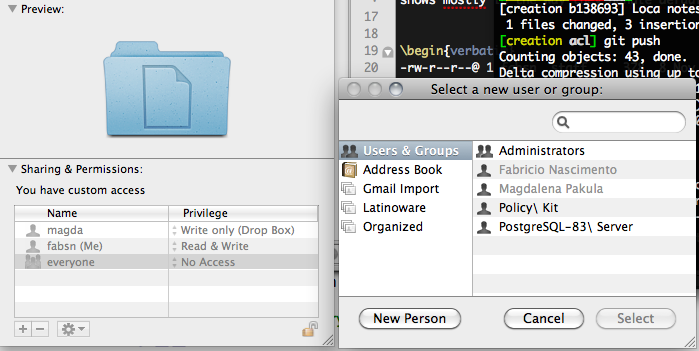
\includegraphics[height=3in]{img/mac-acl.png}
	\caption{Mac OSX Snow Leopard ACL Interface}
	\label{fig:img_mac-acl}
\end{figure}


%A voir maintenant

\subsection*{Using ACL in Linux}


%References 
Les dernière version des distribution Debian ou Ubuntu, comme Ubuntu 9.10, dèjá vient avec le supporte aux ACL. Dans le Ubuntu 8.10 l'application Nautilus, qui est responsable pour la visualisation du système de fichier contenait une interface pour les ACL, apparentement l'interface a été discontinue et le Nautilus du Ubuntu 9.10 n'en y a pas encore. Les pas pour ajouter le supporte dans le Ubuntu 9.10 sont:

\begin{verbatim}
Installer le paquet des acl. 
user@ubuntu:$ sudo apt-get install acl
 
Ajouter le option 'acl' au système de fichier correcte dans le /etc/fstab, comment:
UUID='gros sequence' /dev/hda6 /home ext3 rw,auto,acl 0 1

Remounter le systeme de fichier avec le nouvelle option

user@ubuntu:$ sudo mount /home -o remount

\end{verbatim}

\subsection*{Ajouter ACL aux fichiers}

On peut utiliser le commande 'ls -la' pour regarde les permission. Si une fichier contient information de sécurité avancée (comment access list) on va voir le "character" '+', comment dans le sortie du command 'ls' ci-dessous (\ref{verb:ls}). Une fichier avec '@' était dire que le fichier a quelque EAs. 

\begin{center}
\label{verb:ls}
\begin{verbatim}
-rw-r--r--@ 1 fabsn  staff     378  8 Nov 15:29 Makefile
-rw-r--r--@ 1 fabsn  staff     618  8 Nov 15:59 README
-rw-r--r--@ 1 fabsn  staff      31  8 Nov 15:15 draft-header
-rw-r--r--@ 1 fabsn  staff      24  8 Nov 15:15 header
drwxr-xr-x@ 2 fabsn  staff     102  8 Nov 15:26 img
-rw-r--r--  1 fabsn  staff     972  8 Nov 15:57 rapport-draft.aux
-rw-r--r--  1 fabsn  staff   18129  8 Nov 15:57 rapport-draft.log
drwxrwxr-x+ 3 fabsn  staff	  1024  8 Nov 20:23 repertoire
\end{verbatim}
\end{center}

Pour voir les ACL on doit utilise le commande \emph{getfacl}. Regarde que les information sont ajoute d'accord avec les définition dans l'introduction sur les ACL dans la tabelle \ref{tab:entree}. 

\begin{verbatim}
fabsn@vadmin:/media/esisar$ getfacl repertoire/
# file: repertoire/
# owner: root
# group: root
user::r-x
user:daemon:rwx
user:bin:rwx
user:fabsn:rwx
user:nobody:rwx
group::r-x
group:admin:rwx
group:fabsn:rwx
mask::rwx
other::r-x	
\end{verbatim}

Aussi on a le commande \emph{setfacl} pour modifier, ou ajouter les permission ACL. Le commande dessous par exemple modifie (-m) les permission du utilisateur \emph{fabsn} pour le répertoire. 

\begin{verbatim}
setfacl -m u:fabsn:r-x repertoire
\end{verbatim}

\subsection*{Exemple}

HERE COMES THE EXAMPLE :-).

